\chapter{Executive Summary}
\label{ch:exec-overall}

%%%%%%%%%%%%%%%%%%%%%%%%%%%%%%%%%%%%%%%%%%%%%%%%%%%%%%%%%%%
\section{Overview}
\label{sec:exec-overall-1}

The \dword{dune} will be a world-class neutrino observatory and nucleon decay detector designed to answer fundamental questions about elementary particles and their role in the universe. The international \dword{dune} experiment, hosted by the U.S. Department of Energy's \dword{fnal}, will consist of a \dword{fd} located approximately \SI{1.5}{km} underground at the \dword{surf} in South Dakota, USA, \fixme{I've already seen the abbreviation US (U.S.) used elsewhere in this introduction. This must be consistent across the document. Nora} \SI{1300}{\km} from \dword{fnal}, and a \dword{nd} located on site at \dword{fnal} in Illinois. The far detector will be a very large, modular \dword{lartpc} with a \fdfiducialmass (\SI{40}{\giga\gram}) fiducial mass of \dword{lar}. The \dword{lar} technology 
can uniquely reconstruct neutrino interactions with image-like precision and unprecedented resolution. 

The \dword{dune} detectors will be exposed to the world's most intense neutrino beam originating at \dword{fnal}{}. The high-precision \dword{nd}, \SI{574}{m} from the neutrino source on the \dword{fnal} site, will be used to characterize the intensity and energy spectrum of this wide-band beam. The ability to compare the energy spectrum of the neutrino beam between the \dword{nd} and \dword{fd}
is crucial for discovering new phenomena in neutrino oscillations. The \dword{lbnf}, also hosted by \dword{fnal}, provides the infrastructure for this complex system of detectors at the Illinois and South Dakota sites. \dword{lbnf} is responsible for the neutrino beam, the deep-underground site, and the infrastructure for the \dword{dune} detectors. 

\begin{dunefigure}[DUNE collaboration global map]{fig:map2}{The international \dword{dune}
collaboration. Countries with \dword{dune} membership are in orange.}
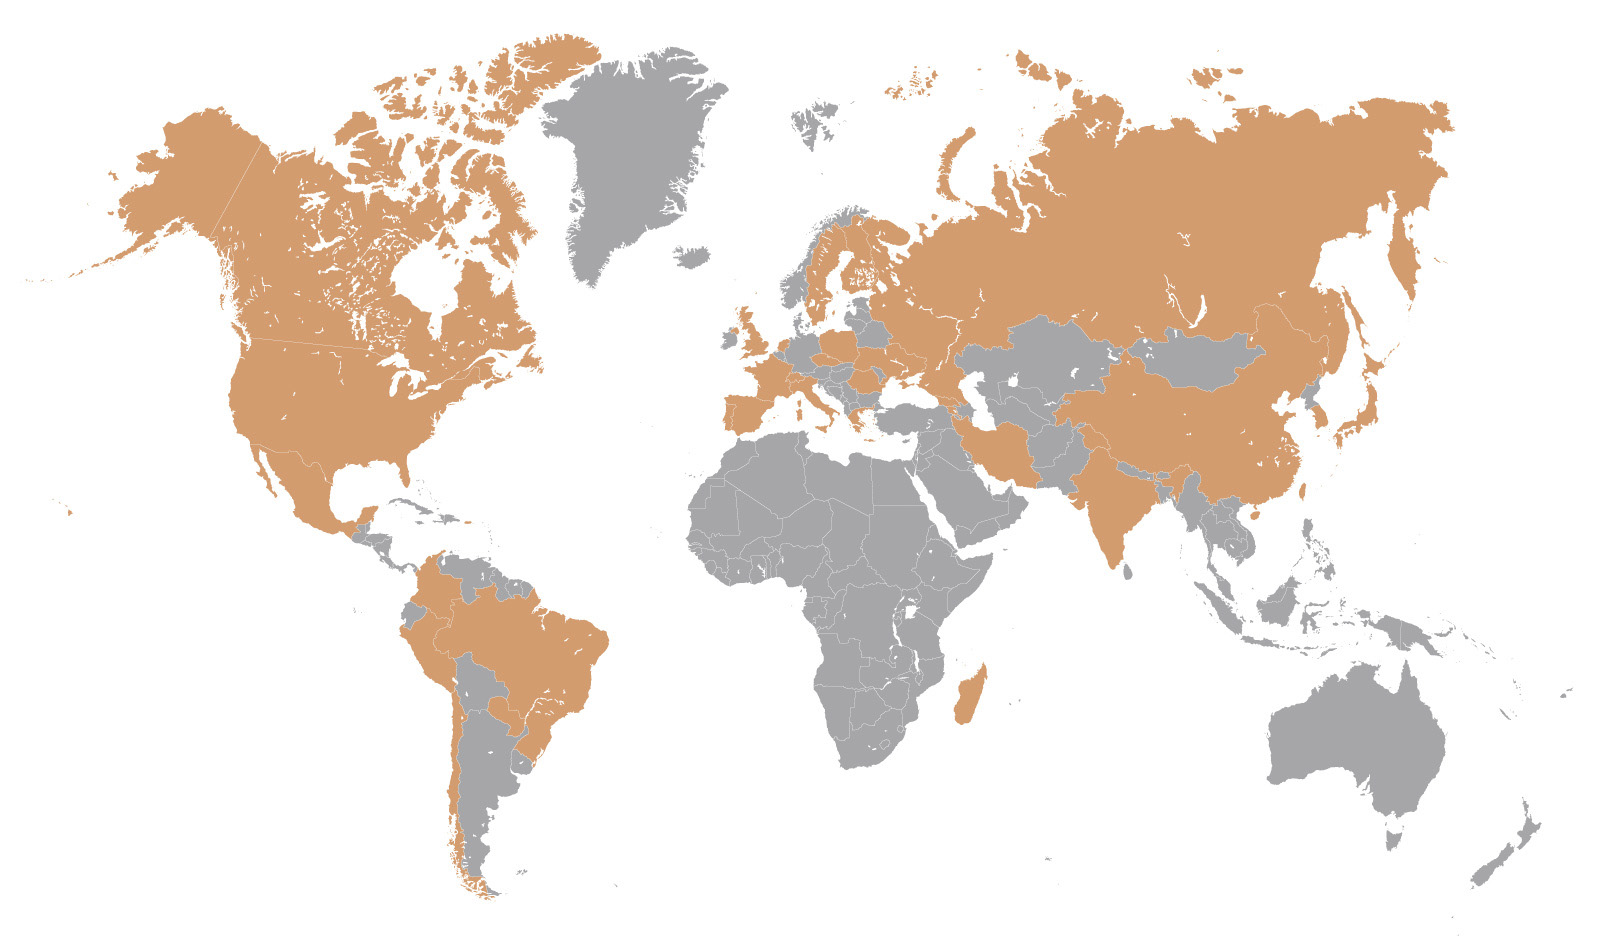
\includegraphics[width=0.9\textwidth]{dune-countries-july2019.jpg}  
\end{dunefigure} %updated by anne 7/15

The \dword{dune} collaboration is a truly global organization with more than \num{1000} scientists and engineers from \num{31} countries (Figure~\ref{fig:map2}). It represents the culmination of several worldwide efforts that developed independent paths toward a next-generation \dword{lbl} neutrino experiment over the last decade. \dword{dune} was formed in April 2015, combining the strengths of the \dword{lbne} project in the USA and the \dword{lbno} project in Europe, adding many new international partners in the process. \dword{dune} thus represents the convergence of a substantial fraction of the worldwide neutrino-physics community around the opportunity provided by the large investment planned by the U.S. \dword{doe} and \dword{fnal} to support a significant expansion of the underground infrastructure at \dword{surf} in South Dakota and to create a megawatt neutrino-beam facility at \dword{fnal} by 2026. 
The \dword{pip2} accelerator upgrade at \dword{fnal}~\cite{pip2-2013} will provide the world's most intense beam of neutrinos for use by the %to the international \dword{lbnf}/
\dword{dune} experiment, enabling a broad physics research program.  
The \dword{pip2} project will deliver between \SIrange{1.0}{1.2}{\MW} of proton beam power from the \dword{fnal} Main Injector in the energy range \SIrange{60}{120}{\GeV} at the start of \dword{dune} and provide a platform for extending beam power to \dword{dune} to multi-MW capability. % (>\SI{2}{\MW}). 
The continuous-wave-compatible, modern superconducting rf linac of \dword{pip2} will increase the reliability of the \dword{fnal} accelerator complex and provide flexibility through customized  beams tailored to specific scientific needs.  

The \dword{lbnf}/\dword{dune} strategy presented in this \dword{tdr} has been developed to meet the requirements set out in the report of the Particle Physics Project Prioritization Panel (P5) in 2014. It also takes into account the recommendations of the \dword{espp} adopted by the \dword{cern} Council in 2013, which classified the \dword{lbl} neutrino program as one of the four scientific objectives that require international infrastructure.

The P5 report~\cite{p5report} set the goal of reaching a sensitivity to \dword{cpv} of more than three standard deviations (\num{3}$\sigma$) over more than $75\%$ 
of the range of possible values of the unknown \dshort{cp}-violating phase \deltacp.
Based partly on this goal, the report stated that ``the 
minimum requirements to proceed are the identified capability to reach an exposure 
of \num{120}~\ktMWyr{} by the 2035 time frame, the far detector situated underground 
with cavern space for expansion to at least \fdfiducialmass \dword{lar} fiducial volume, and \SI{1.2}{MW} 
beam power upgradeable to multi-megawatt power.
The experiment should have the demonstrated 
capability to search for \dwords{snb} and for proton decay, providing a significant 
improvement in discovery sensitivity over current searches for the proton lifetime.'' The strategy and design presented in this \dword{tdr} meet these requirements.

This multi-volume document is the \dword{tdr} for the \dword{dune} \dword{fd} and covers the technology choices for the first three far detector modules. The type of \dword{lar} 
technology used for the fourth module remains to be decided. The \dword{tdr} should provide a clear statement of the physics goals of the \dword{dune} collaboration and describe the detector designs that we believe will achieve these goals. The \dword{tdr} includes dedicated volumes on the \dword{dune} physics program, the \dword{dune} \dwords{fd}, and the \dword{dune} \dword{tc} organization. In addition to overviews of the other volumes, this executive summary volume also includes dedicated chapters on the \dword{nd} and computing, which will be the subject of future \dwords{tdr}.

\section{Primary Science Goals}


The \dword{dune} experiment will combine the world's most intense neutrino beam, a deep underground site, massive \dword{lar} detectors, and an  \dword{nd}  capable of enabling a broad science program to address some of the most fundamental questions in particle physics. 
The primary science goals of \dword{dune}, described in detail in Volume~\volnumberphysics{}, \voltitlephysics{}, are to 
\begin{itemize}

\item carry out a comprehensive program of neutrino oscillation measurements using \numu and \anumu beams from \dword{fnal}. This program includes measuring the  \dword{cp} phase $\deltacp$, determining the neutrino mass ordering (the sign of \dm{31}$ \equiv m_3^2-m_1^2$), measuring the mixing angle $\theta_{23}$, and  determining the octant in which this angle lies,
as well as conducting sensitive tests of the three-neutrino paradigm. Paramount among these is the discovery of \dword{cp} violation in neutrino oscillations, which may give insight into the origin of the matter-antimatter asymmetry in the universe, one of the fundamental questions in particle physics and cosmology. 

\item detect and measure the $\nu_\text{e}$ flux from a core-collapse supernova within our galaxy, should one occur during the lifetime of the \dword{dune} experiment. Such a measurement would provide a wealth of unique information about the early stages of core collapse and could signal the birth of a black hole.
    
\item search for proton decay in important decay modes and for other baryon-number-violating processes. The observation of baryon number violation would represent a ground-breaking discovery in physics, providing a key requirement for a grand unification of the forces. 

\end{itemize}

The intense neutrino beam from \dword{lbnf}, the massive \dword{dune} \dword{lartpc} \dword{fd}, and the high-resolution
\dword{dune} \dword{nd} will also provide a rich ancillary science program beyond the primary goals of the experiment. The ancillary science program includes
\begin{itemize}
     \item other accelerator-based neutrino flavor transition measurements with sensitivity to \dword{bsm} physics, such as \dword{nsi}, Lorentz violation,  violation of the \dword{cpt}, the existence of sterile neutrinos, large extra dimensions, and heavy neutral leptons;
     \item measurements of tau neutrino appearance;
     \item measurements of neutrino oscillation phenomena using atmospheric neutrinos;
     \item a rich neutrino interaction physics program using the \dword{dune} \dword{nd}, including a wide range of measurements of neutrino cross sections and studies of nuclear effects; 
     \item  searches for dark matter.
\end{itemize} 
Further advances in \dword{lartpc} 
technology during \dword{dune} \dword{fd} construction may open up the opportunity
to observe very low-energy phenomena such as solar neutrinos or even the diffuse supernova neutrino flux.


%%%%%%%%%%%%%%%%%%%%%%%%%%%%%%%%%%%%%%%%%%%%%%%%%%%%%%%%%%%%%%%
\section{The LBNF Facility} 

The \dword{lbnf} project is building a facility in South Dakota that will house and provide infrastructure for the first two \dword{dune} \dword{fd} modules and the \dword{nd} in Illinois.  Figure~\ref{fig:lbnf} shows
a schematic of the facilities at the two sites, and Figure~\ref{fig:caverns} shows a diagram of the cavern layout for the \dword{fd}.  
The organization and management of \dword{lbnf} is separate from the \dword{dune} collaboration. \dword{lbnf} is also hosted by \dword{fnal}, and its design and construction are organized as a \dword{doe}/\dword{fnal} project incorporating international partners. 


%The organization and management of \dword{lbnf}, hosted by \dword{fnal}{}, is separate from the \dword{dune} collaboration, intended to enable constructing and operating the \dword{dune} detectors in South Dakota and Illinois. %\fixme{unclear and repetitive}The \dword{dune} collaboration will construct a deep-underground neutrino observatory in South Dakota using four independent \dword{lar} \dword{tpc} modules of 10 kt fiducial massand a high-precision, movable \dword{nd} at \dword{fnal} comprising an \dword{lar} \dword{tpc}, a gas-argon \dword{tpc}, and a beam spectrometer. To enable the scientific program for the \dword{dune} experiment,\dword{lbnf} will provide the facilities in Illinois and South Dakota.These facilities are geographically separated into the near site facilities, to be constructedat \dword{fnal}, and the far site facilities, located at \dword{surf}. Figure~\ref{fig:lbnf} showsa schematic of the facilities at the two sites, and Figure~\ref{fig:caverns} shows a diagram of the cavern layout. 


\begin{dunefigure}[ 	
LBNF/DUNE project: beam from Illinois to South Dakota]{fig:lbnf}{ 	
LBNF/DUNE project: beam from Illinois to South Dakota.}
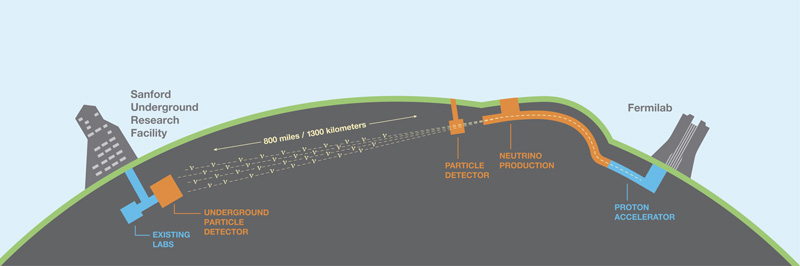
\includegraphics[width=0.9\textwidth]{lbnf_dune_graphic_miles_km-15-0031-01.jpg}
%\label{fig:mhexec}
\end{dunefigure}

\begin{dunefigure}[ 	
Underground caverns for DUNE in South Dakota]{fig:caverns}{Underground caverns for the \dword{dune}{} \dword{fd}{} and cryogenics systems at \dword{surf} in South Dakota. The drawing, which looks northeast, shows the first two far detector modules in place.}
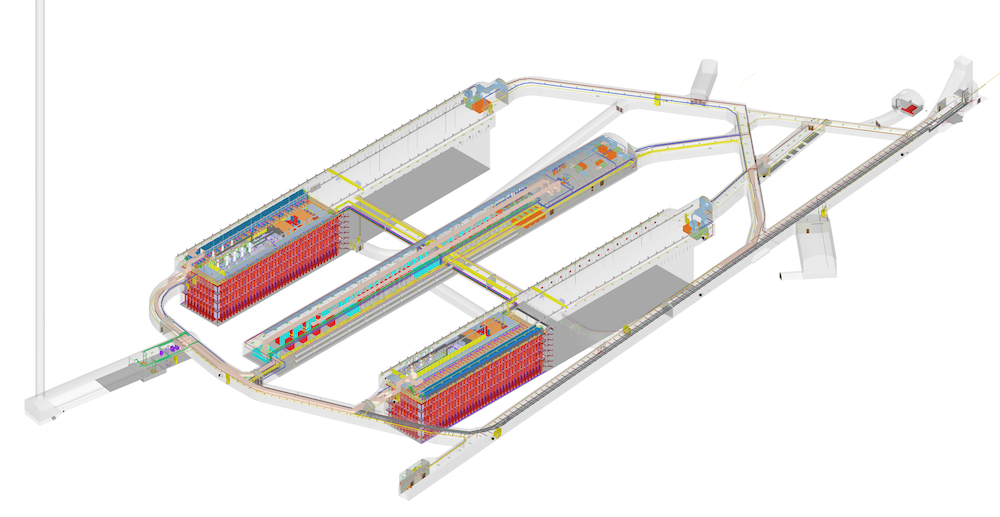
\includegraphics[width=0.99\textwidth]{caverns_full_assembly}
\end{dunefigure}


%Specifically, \dword{lbnf} provides
The \dword{lbnf} project provides to \dword{dune}
\begin{itemize}
\item  the  technical and conventional facilities for a powerful neutrino beam using the \dword{pip2} upgrade~\cite{pip2-2013} of the \dword{fnal} accelerator 
complex. The \dword{pip2} project will deliver between \SIrange{1.0}{1.2}{MW} of proton beam power from \dword{fnal}'s Main Injector in the energy range  \SIrange{60}{120}{GeV} at the start of \dword{dune} operations as well as a platform for extending beam power to \dword{dune} to %multi-MW capability (
$>\,$\SI{2}{MW}. %). 
A further planned upgrade 
of the accelerator complex will provide up to \SI{2.4}{\MW} of beam power by 2030. 

\item  the civil construction, or \dword{cf}, for the \dword{nd} systems at \dword{fnal}; (see Figure~\ref{fig:beamline});

\item the excavation of three underground caverns at \dword{surf} to house the \dword{dune} \dword{fd}. The north and south caverns will each house two cryostats, each with a
 minimum \nominalmodsize fiducial mass of liquid argon, while the \dword{cuc} will house cryogenics and data acquisition facilities for all four detector modules;

\item surface, shaft, and underground infrastructure to support 
outfitting the caverns with four free-standing, steel-supported cryostats 
and the required cryogenics systems for rapidly deploying the first two \nominalmodsize \dword{fd} modules. 
The intention is to install the third and fourth cryostats as rapidly as funding will 
allow.

\end{itemize}


\begin{dunefigure}[Neutrino beamline and DUNE near detector hall in Illinois
]{fig:beamline}{Neutrino beamline and \dword{dune}{} near detector hall at \dword{fnal}{} in Illinois}
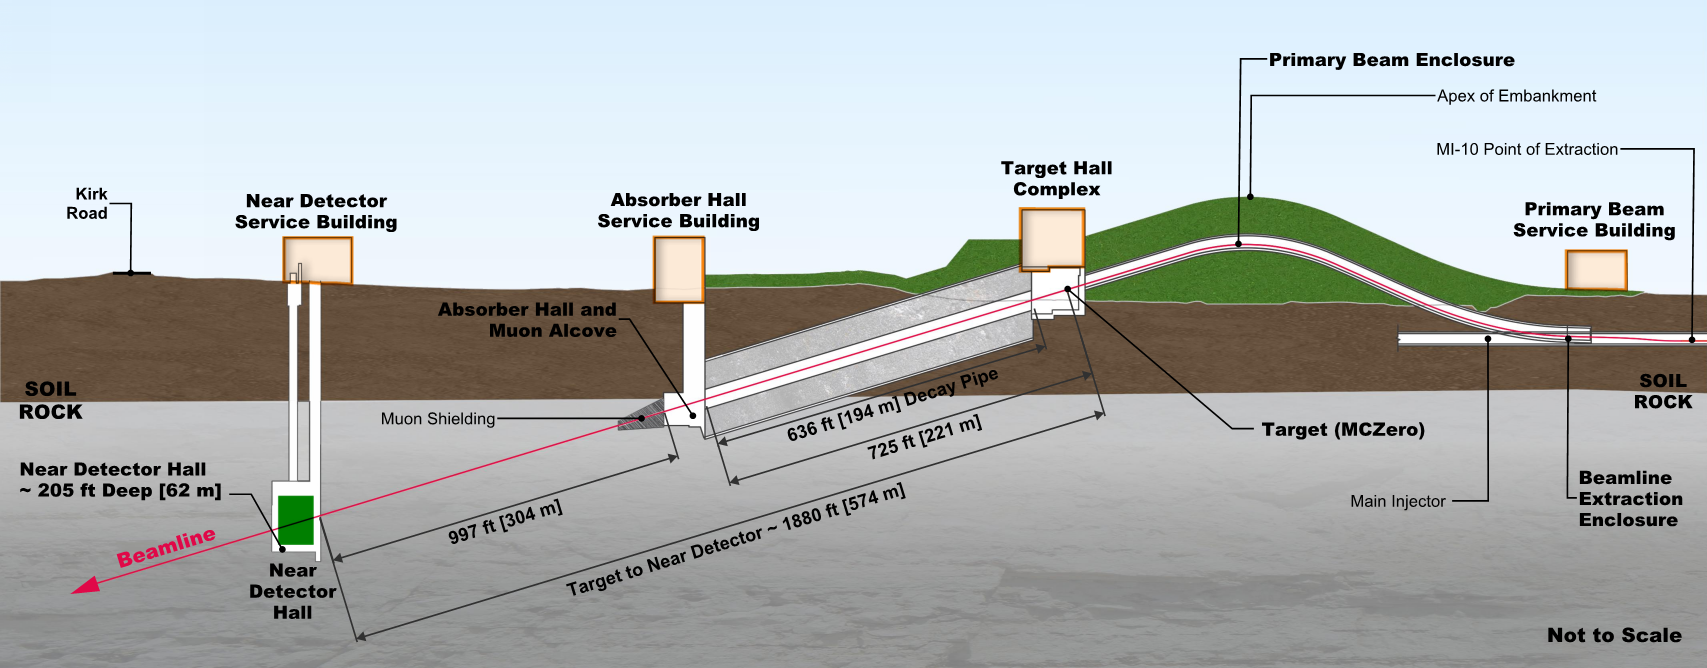
\includegraphics[width=0.95\textwidth]{beamline-sideview.jpg}
\end{dunefigure}



\section{The DUNE Experiment}

The \dword{dune} experiment includes a precision \dword{nd} at the edge of the \dword{fnal} site, in Batavia, Illinois, and a very large, modular \dword{fd} approximately \SI{1.5}{km} underground at \dword{surf} in Lead, South Dakota, \SI{1300}{km} (\SI{800}{miles}) from \dword{fnal}. The \dword{dune} \dword{fd} is the focus of this \dword{tdr}. 

% ecb: Do ProtoDUNEs show up here or in a separate section? Somewhere, we need to state what specific performance measures we are counting on having from ProtoDUNE before the TDR.

\subsection{Far Detector}
\label{ch:dune-det-tech-ov-fd}

The \fdfiducialmass \dword{dune} \dword{fd} consists of four \dword{lartpc} \dwords{detmodule}, each with fiducial mass of at least \nominalmodsize, installed approximately \SI{1.5}{km} underground. The \dword{lartpc} technology provides
excellent tracking and calorimetry performance, making it an ideal
choice for the \dword{dune} \dword{fd}. Each \dword{lartpc} fits inside a cryostat of internal dimensions
\cryostatwdth (W) $\times$ \cryostatht (H) $\times$ \cryostatlen~(L) containing a total \dword{lar} mass of about \larmass{}.
 The four identically sized modules are sufficiently flexible for staging construction and  evolving \dword{lartpc} technology.

\dword{dune} is planning for and prototyping two \dword{lartpc} technologies:
\begin{itemize}
\item \Dword{sp}: In the \dword{sp} technology, ionization charges are drifted horizontally in \dword{lar} and read out on wires in the liquid.  The maximum drift length in the first \dword{dune} \dword{spmod} is \spmaxdrift, and the nominal drift field is \spmaxfield, corresponding to a cathode \dword{hv} of \sptargetdriftvoltpos. This design requires very low-noise electronics to achieve readout with good \dword{s/n} because no signal amplification occurs in the liquid. This technology was pioneered in the \dword{icarus} project, and after several decades of worldwide R\&D, is now a mature technology. It is the technology used for \dword{fnal}'s currently operating \dword{microboone} detector, as well as the \dword{sbnd} detector, which is under construction. 

\item \Dword{dp}: This technology was pioneered at a large scale by the \dword{wa105} collaboration at \dword{cern}. It is less established than the \dword{sp} technology but offers several advantages and challenges. Here, ionization charges drift vertically in \dword{lar} and are transferred into a layer of gas above the liquid. Devices called \dwords{lem} amplify the signal charges  in the gas phase. The gain achieved in the gas reduces stringent requirements on the electronics and increases the possible drift length, which, in turn, requires a correspondingly higher voltage. The nominal drift field is \dpnominaldriftfield, as for the \dword{sp} detector, but corresponds to a cathode \dword{hv} of \dptargetdriftvoltpos.
The maximum drift length in the \dword{dpmod} is \dpmaxdrift{}.  
\end{itemize}
In both technologies, the drift volumes are surrounded by a \dword{fc} that defines the active detector volume and ensures uniformity of the \efield to 1\% within that volume.

Argon is an excellent scintillator at a wavelength of \SI{127}{\nano\meter}. This fast scintillation light, once shifted into the visible spectrum, is collected by \dwords{pd} in both designs. The \dwords{pd} provide a time $t_{0}$ for every event, indicating when the ionization electrons begin to drift. Comparing the time at which the ionization signal reaches the anode relative to the $t_{0}$ allows reconstructing event topology in the drift coordinate; the precision of the measured $t_{0}$, therefore, directly corresponds to the precision of the spatial reconstruction in this direction. 

Two key factors affect the performance of the \dword{dune} \dwords{lartpc}.  First, the \dword{lar} purity must be high enough to achieve minimum charge attenuation over the longest drift lengths in a given \dword{detmodule}.  Thus, the levels of electronegative contaminants (e.g., oxygen and water) must be maintained at \dword{ppt} levels.  The \dword{sp} and \dword{dp} designs have slightly different purity requirements (expressed in minimum electron lifetimes of \SI{3}{ms} versus \SI{5}{ms}) due to the different drift lengths.

Second, the electronic readout of the \dword{lartpc} requires very low noise levels to allow the signal from the drifting electrons to be clearly discerned over the baseline of the electronics.  This requires using low-noise cryogenic electronics. 

The plans for the \dword{sp} and \dword{dp} \dwords{tpc} are described briefly in the following sections, more fully in Chapters~\ref{ch:exec-sp} and~\ref{ch:exec-dp}, and finally in great detail in Volumes~\volnumbersp{} and~\volnumberdp{} of this \dword{tdr}. 
The \dword{dune} collaboration is committed to deploying both technologies. 
For planning, we assume that the first \dword{detmodule} will be
\dword{sp}, and the second will be \dword{dp}.
The actual sequence of \dword{detmodule} installation will depend on results from the prototype detectors, described below, and on available resources.

The full \dword{dune} \dword{fd} requires four modules. For the \dword{tdr}, we will describe plans for the first three modules: two \dwords{spmod}, one of which will be the first module installed, and one \dword{dpmod}. Resources for the fourth \dword{detmodule}, which may use a more advanced design, remain to be identified. 

%%%%%%%%%%%%%%%%%%%%%%%%%%%%%%%%%%%%%%%%
\subsubsection{Single-Phase Technology}
\label{sec:fdsp-exec-splar}

Figure~\ref{fig:LArTPC1ch1} shows the general operating principle of the \dword{sp} \dword{lartpc}, as previously demonstrated by  \dword{icarus}~\cite{Icarus-T600}, \dword{microboone}~\cite{microboone}, \dword{argoneut}~\cite{Anderson:2012vc}, \dword{lariat}~\cite{Cavanna:2014iqa}, and \dword{protodune}~\cite{Abi:2017aow}. Figure~\ref{fig:DUNESchematic1ch1} shows the configuration of a \dword{dune} \dword{spmod}. Each of the four drift volumes of \dword{lar} is subjected to a strong electric field (\efield{}) of \spmaxfield. Charged particles passing through the \dword{tpc} ionize the argon, and the ionization electrons drift in the \efield to the anode planes. 


\begin{dunefigure}[The SP LArTPC operating principle]{fig:LArTPC1ch1}
{The general operating principle of the \dword{sp} \dword{lartpc}.}
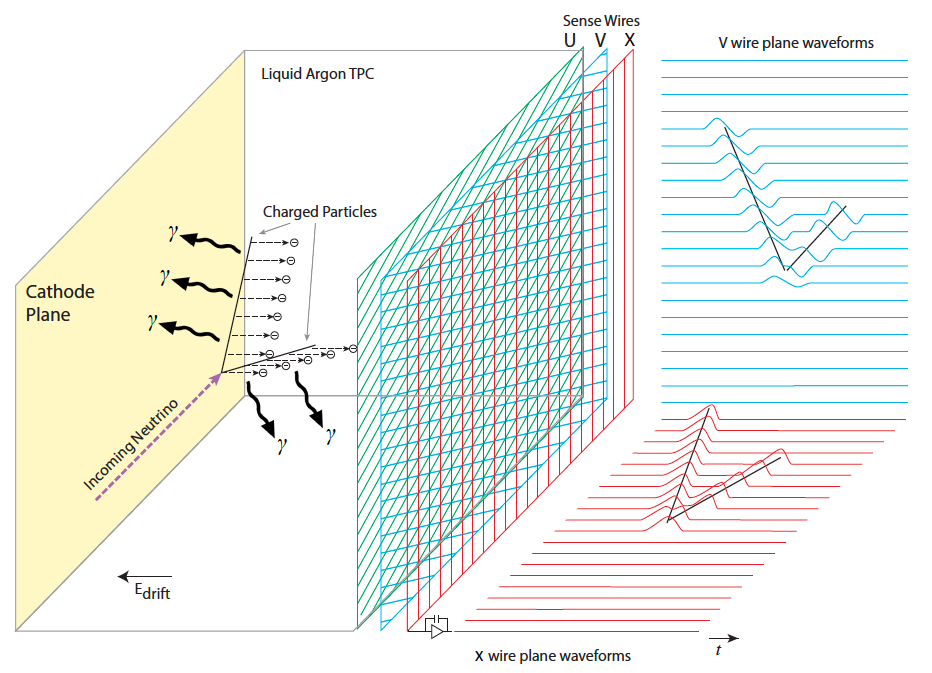
\includegraphics[width=0.75\textwidth]{TheBoPicture.png} 
\end{dunefigure}

\begin{dunefigure}[A \nominalmodsize DUNE far detector SP module]{fig:DUNESchematic1ch1}
{Schematic of a \nominalmodsize \dword{dune} \dword{fd} \dword{spmod}, showing the alternating anode (A) and cathode (C) planes that divide the \dword{lartpc} into four separate drift volumes. The red arrows point to one top and one bottom \dword{fc} module and to the rear endwall field cage.}
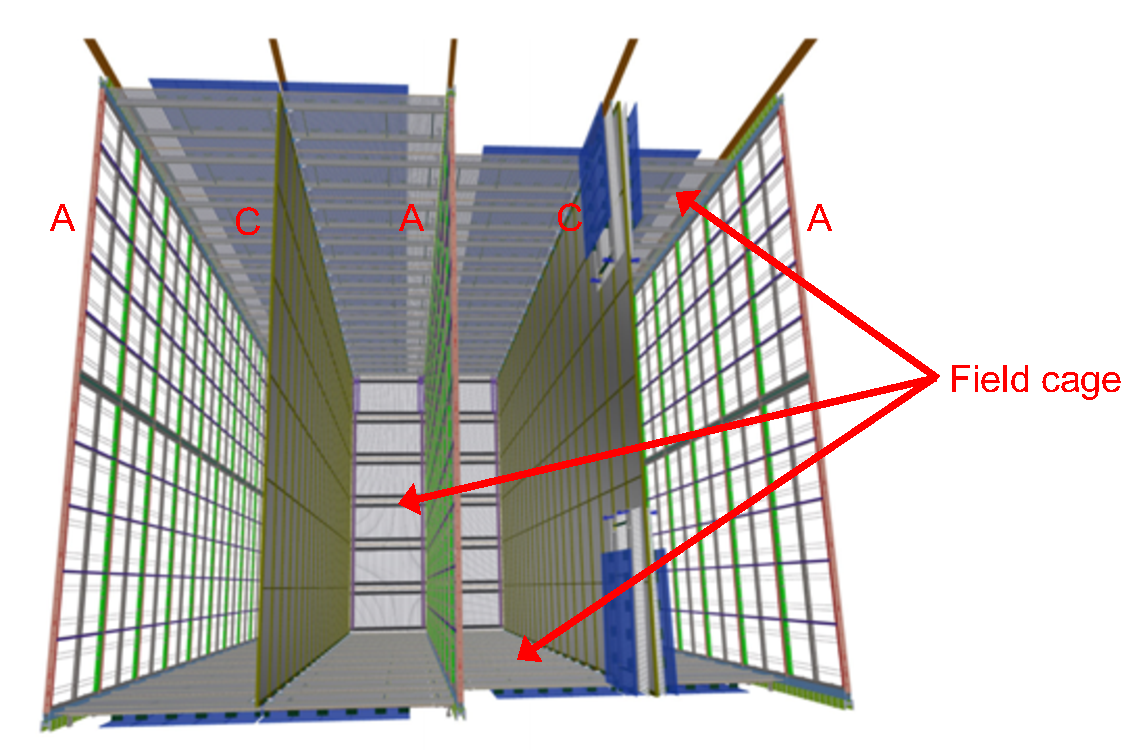
\includegraphics[width=0.65\textwidth]{DUNESchematic.pdf}
\end{dunefigure}

An \dword{spmod} is instrumented with three module-length anode planes constructed from \SI{6}{m} high by \SI{2.3}{m} wide \dwords{apa}, stacked two \dword{apa}s high and 25 wide, for 50 \dword{apa}s per plane, or 150 total. Each \dword{apa} has three layers of active wires forming a grid. The relative voltage between the layers is chosen to ensure transparency to the drifting electrons of the first two layers ($U$ and $V$). These layers produce bipolar induction signals as the electrons pass through them. The final layer ($X$) collects the drifting electrons, resulting in a unipolar signal. The pattern of ionization collected on the grid of anode wires provides the reconstruction in the remaining two coordinates perpendicular to the drift direction.



Novel \dword{pd} light collector modules (called ARAPUCAs) using \dwords{sipm} are placed in the inactive space between the innermost wire planes of the \dwords{apa}, installed through slots in a pre-wound \dword{apa} frame. 
Each \dword{apa} has ten \dword{pd} modules for a total of \num{1500} per \dword{spmod}.  Of these, \num{500} are mounted in central \dword{apa} frames and must collect light from both directions, 
and \num{1000} are mounted in frames  near the %vessel 
cryostat walls and collect light from only one direction. 

\FloatBarrier
%%%%%%%%%%%%%%%%%%%%%%%%%%%%%%%%%%%%%%%%
\subsubsection{Dual-Phase Technology}
\label{sec:fddp-exec-splar}

The \dword{dp} operating principle, illustrated in Figure~\ref{fig:DPprinciplech1}, is very similar to that of the \dword{sp}. % design. 
 Charged particles that traverse the active volume of the \dword{lartpc} ionize the medium while also producing scintillation light.  The ionization electrons drift along an \efield toward a segmented anode where they deposit their charge and where  \dwords{pd} pick up the scintillation light. 
 
 
\begin{dunefigure}[The DP LArTPC operating principle]{fig:DPprinciplech1}{The general operating principle of the \dword{dp} \dword{lartpc}.}
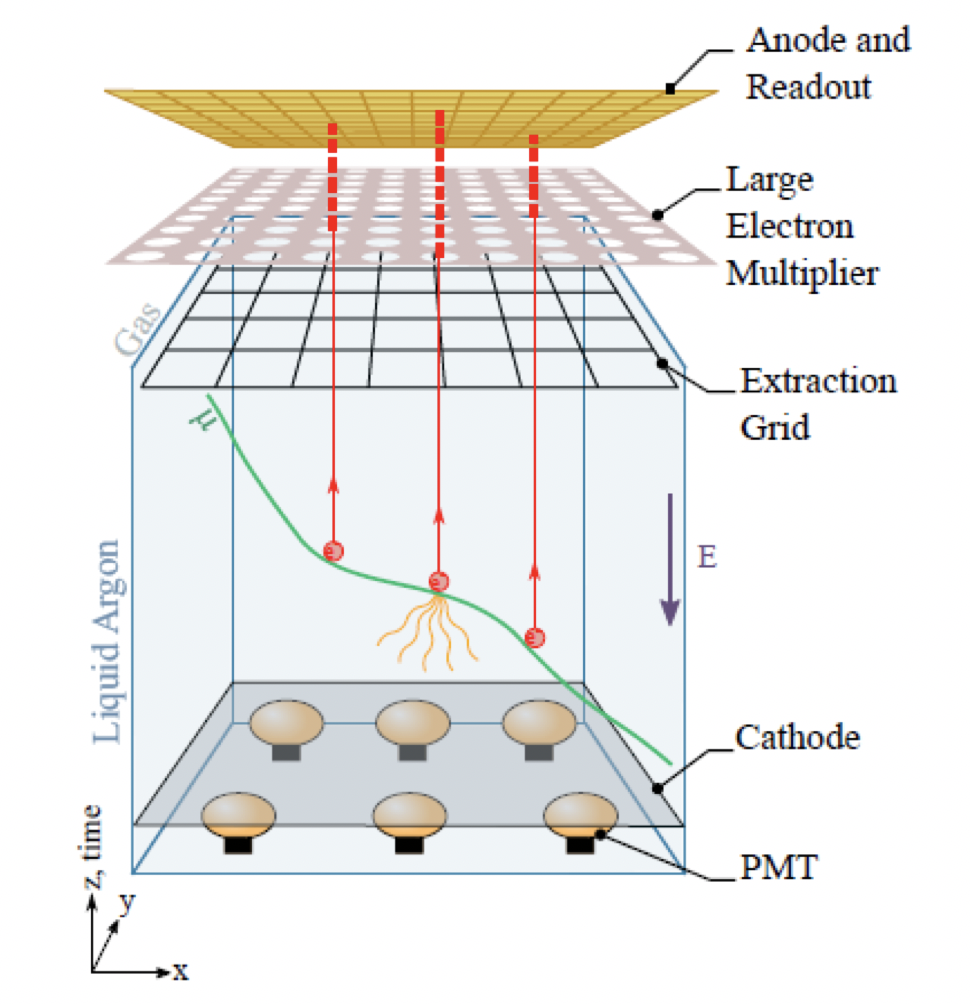
\includegraphics[width=0.5\textwidth]{dualphase-principle}
\end{dunefigure}

%The key differentiating concept of the \dword{dp} design is the amplification of the ionization signal in an avalanche process that takes place in a layer of argon gas above the \dword{lar}.  
In this design, shown in Figure~\ref{fig:DPdet1ch1}, electrons drift upward toward an extraction grid just below the liquid-vapor interface. 
After reaching the grid, an \efield stronger than the \dpnominaldriftfield{} drift field extracts the electrons from the liquid up into the gas phase. Once in the gas, electrons encounter micro-pattern gas detectors, called \dwords{lem}, with high-field regions. The \dwords{lem} amplify the electrons in avalanches that occur in these high-field regions. The amplified charge is then collected and recorded on a \twod anode
consisting of two sets of %\SI{3.125}{mm}-pitch 
gold-plated copper strips that provide the $x$ and $y$ coordinates (and thus two views) of an event. 

\begin{dunefigure}[A \nominalmodsize DUNE far detector DP module]{fig:DPdet1ch1}
  {Schematic of a \nominalmodsize \dword{dune} \dword{fd} \dword{dp} \dword{detmodule} with cathode, \dwords{pmt}, \dword{fc}, and anode plane with \dwords{sftchimney}.}
  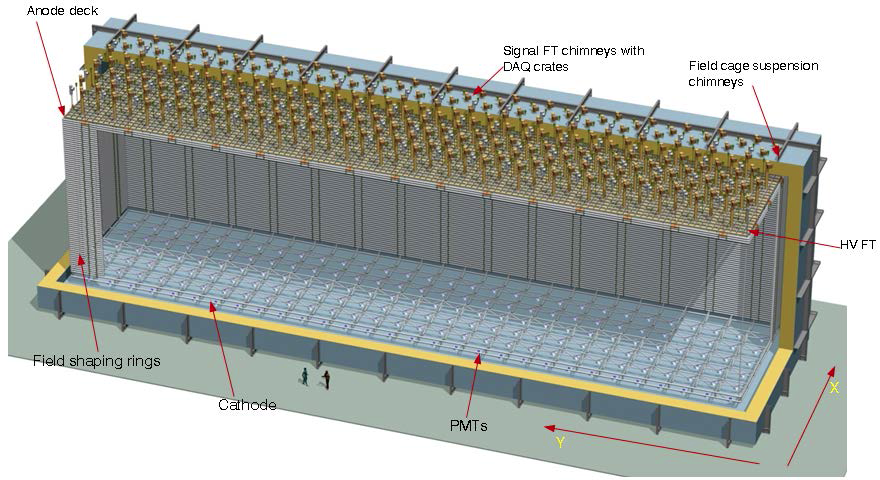
\includegraphics[width=0.9\textwidth]{DUNE-CDR-detectors-volume-optim.png}
\end{dunefigure}

 The extraction grid, \dword{lem}, and anode are assembled into three-layered sandwiches with precisely defined inter-stage distances and inter-alignment,  which are then connected horizontally into \num{9}~m$^2$ modular detection units. These detection units are called \dwords{crp}.

The precision tracking and calorimetry offered by the \dword{dp} technology provides excellent capabilities for identifying interactions of interest while mitigating sources of background.  Whereas the \dword{sp} design has multiple drift volumes, the \dword{dpmod} design allows a single, fully homogeneous \dword{lar} volume with a much longer drift length.

An array of \dwords{pmt} coated with a wavelength-shifting material sits below the cathode. The \dwords{pmt} record  the time and pulse characteristics of the incident light.



\FloatBarrier
%%%%%%%%%%%%%%%%%%%%%%%

\subsubsection{ProtoDUNEs: Far Detector Prototypes}

The \dword{dune} collaboration has constructed 
two large prototype detectors (\dwords{protodune}), \dword{pdsp}, and \dword{pddp}.  %one using \single readout (\dword{pdsp}) and the other \dual readout (\dword{pddp}).
 Each is approximately one-twentieth the size of a \dword{dune} \dword{detmodule} but uses components identical in size to those of the full-scale module. \dword{pdsp} has the same \spmaxdrift maximum drift length as the full \dword{spmod}. \dword{pddp} has a \SI{6}{m} maximum drift length, half that planned for the \dword{dpmod}. See the photographs in figures~\ref{fig:protodunes_northarea} and~\ref{fig:protodunes_interior}.

\begin{dunefigure}[ProtoDUNE cryostats at the CERN Neutrino Platform]
{fig:protodunes_northarea}
{\dword{pdsp}{} and \dword{pddp}{} cryostats in the \dword{cern}{} Neutrino Platform in \dword{cern}'s North Area.}
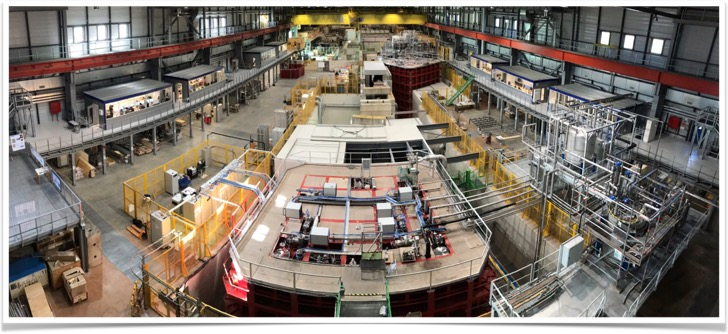
\includegraphics[width=0.9\linewidth]{neutrinoplatform.jpg}
\end{dunefigure}

\begin{dunefigure}[Interior views of the ProtoDUNEs]
{fig:protodunes_interior}
{Interior views of \dword{pdsp}{} (left) and \dword{pddp}{} (right). For \dword{pdsp}{}, one of two identical drift volumes is shown.}
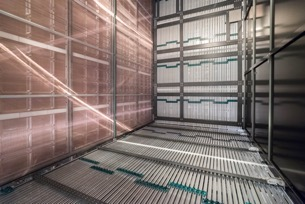
\includegraphics[width=0.46\linewidth]{graphics/ProtoDUNE-sp-interior.jpg}\hspace{0.05\linewidth}
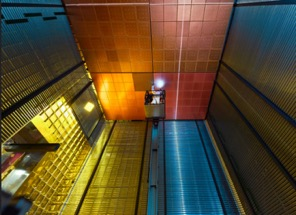
\includegraphics[width=0.44\linewidth]{graphics/protodune-dp-interior.jpg}
\end{dunefigure}

These large-scale prototypes allow us to validate key aspects of the \dword{tpc} designs, test engineering procedures, and collect valuable calibration data using a hadron test beam. The following list includes the key goals of the \dword{protodune} program:
\begin{enumerate}
\item Production of components:
\begin{itemize}
\item stress-testing the production and quality
assurance processes of detector components,
\item mitigating the associated risks for the far detector.
\end{itemize}
\item Validation of installation procedures:
\begin{itemize}
\item testing the interfaces between the detector elements,
\item mitigating the associated risks for the far detector.
\end{itemize}
\item Operating detector with cosmic rays:
\begin{itemize}
\item validating the detector designs and
performance.
\end{itemize}
\item Collecting test beam data:
\begin{itemize}
\item measuring essential physics response of the detector.
\end{itemize}
\end{enumerate}


% -- (ed) I put DP sentence first to get it out of the way before the long SP discussion, but it may be too awkward this way.
 Construction of the \dword{pddp} detector was complete in June of 2019, and the detector should begin collecting cosmic-ray data in August 2019. The construction phase of \dword{pdsp} was finished in July 2018, and the detector was filled with \dword{lar} in August 2018. The detector collected hadron beam data and cosmic rays during the fall of 2018 and continues to collect cosmic-ray data.

The data taken with the \dword{pdsp} detector demonstrates the excellent performance of the detector and has already provided valuable information on the design, calibration, and simulation of the \dword{dune} \dword{fd}. In all, $99.7\%$ of the 15360 \dword{tpc} electronics channels are responsive in the \dword{lar}. The \dword{enc} amounts to $\approx 550$ $e^{-}$ on the collection wires and $\approx 650$ $e^{-}$ on the induction wires. An average \dword{s/n} of 38 for the collection plane is measured using cosmic-ray muons, while for the two induction planes, the \dword{s/n} is 14 (U) and 17 (V), exceeding the requirement of %a ratio $9/1$ 
for the \dword{dune} \dword{fd}. 


Because \dword{pdsp} is located on the surface,  an excess of ions accumulate in the drift volume, % that distorts 
distorting the \efield and the reconstructed particle trajectories; this is known as the space charge effect. % (SCE) \fixme{This abbreviation (SCE) is not in the glossary. Is it necessary to abbreviate space charge effect at all?}. 
A calibration procedure removes the detector non-uniformity, which is dominated by this effect. %the SCE. 
We then convert the charge deposited along the track to the energy loss ($dE/dx$) using stopping cosmic-ray muons. The calibration constants that have been derived with this method are applied to the energy deposits measured for the beam particles, including muons, pions, protons, and positrons.
The resulting $dE/dx$ distributions agree well with expectations.  Figure~\ref{fig:pdtpcpd} (left) shows the calibrated $dE/dx$ values as a function of the track residual range for protons in the 1 GeV/$c$ beam, in good agreement with expectations. 

\begin{dunefigure}[Calibrated $dE/dx$ vs residual range in ProtoDUNE-SP]
{fig:pdtpcpd}
{Calibrated $dE/dx$ versus residual range measured by \dword{tpc} for 1 GeV/c stopping protons (left) and response of ARAPUCA photon-detector module in \dword{apa}{}3 as a function of incident electron kinetic energy (right).} 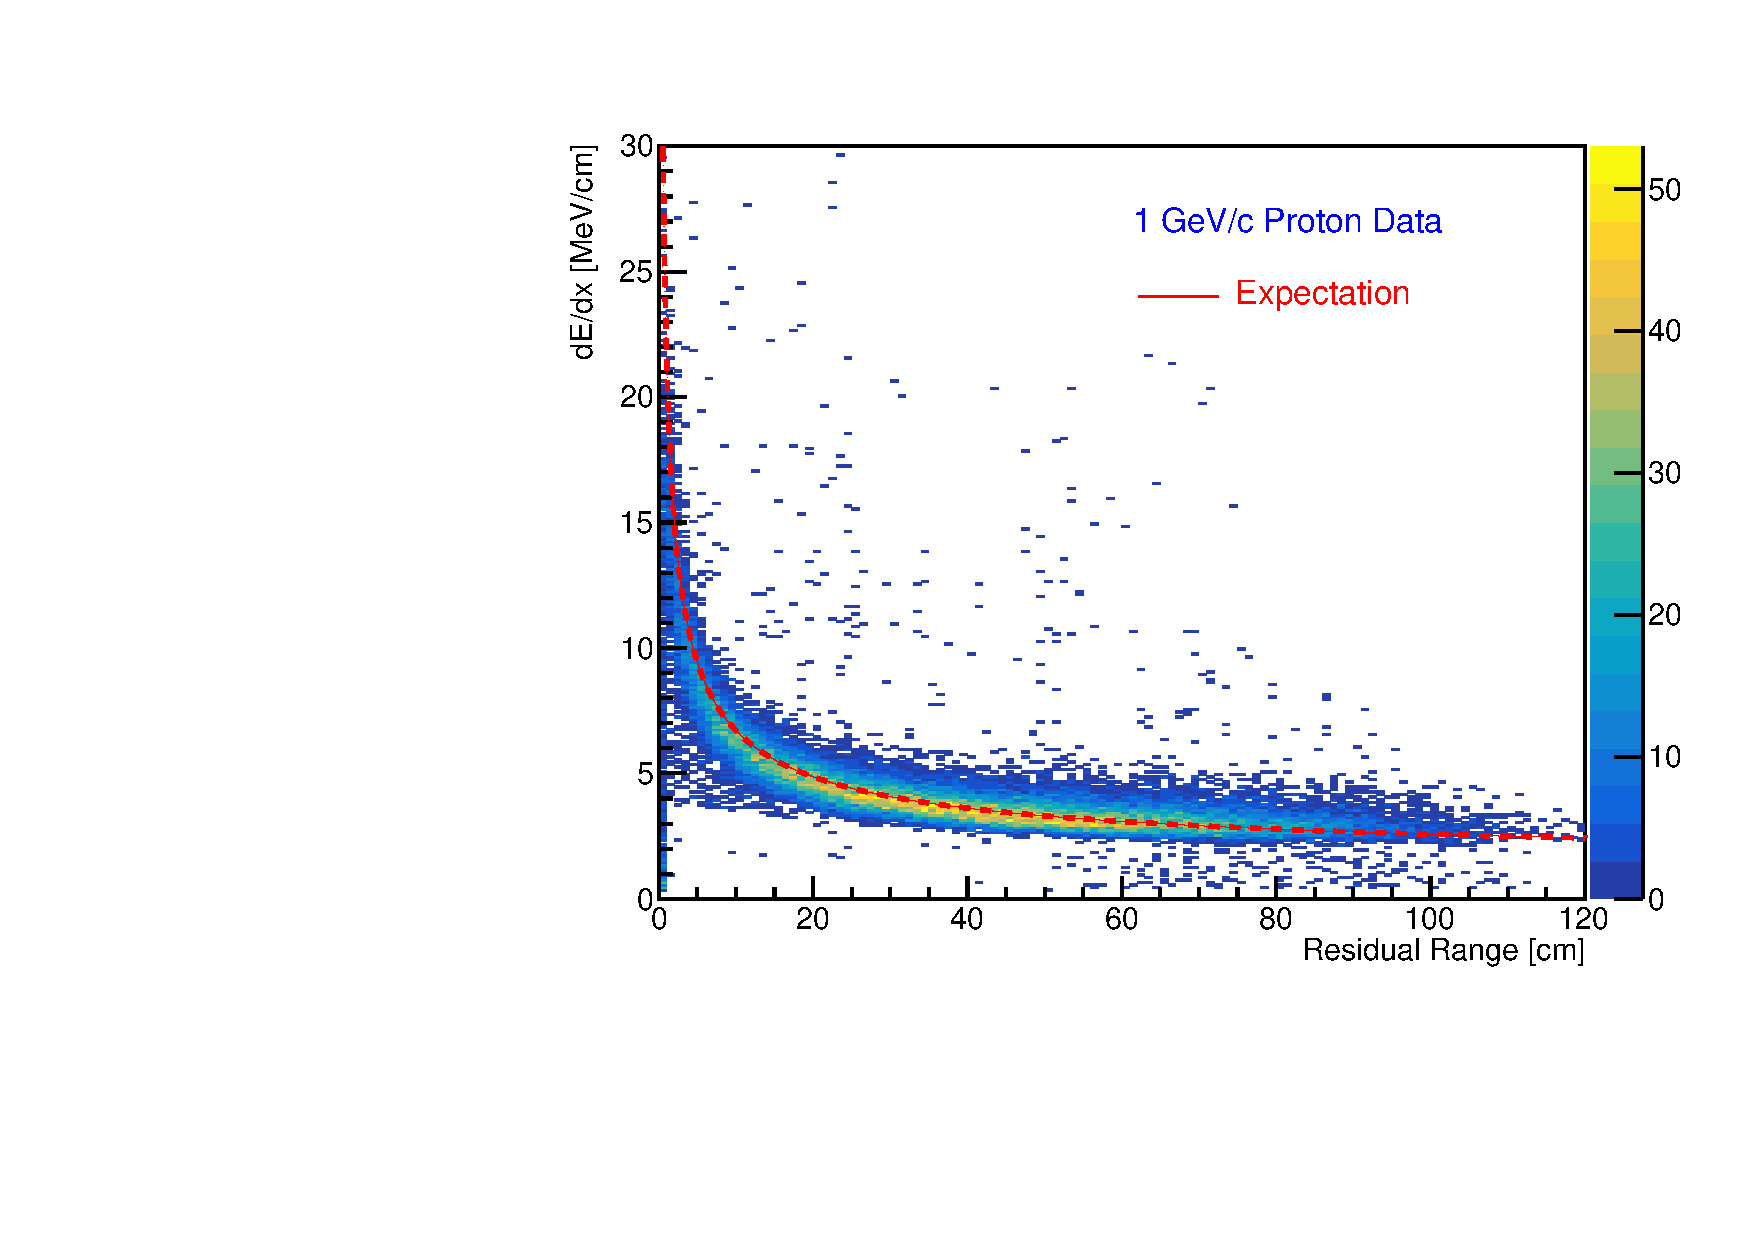
\includegraphics[width=0.47\linewidth]{graphics/dedx_rr_data_v5.pdf}
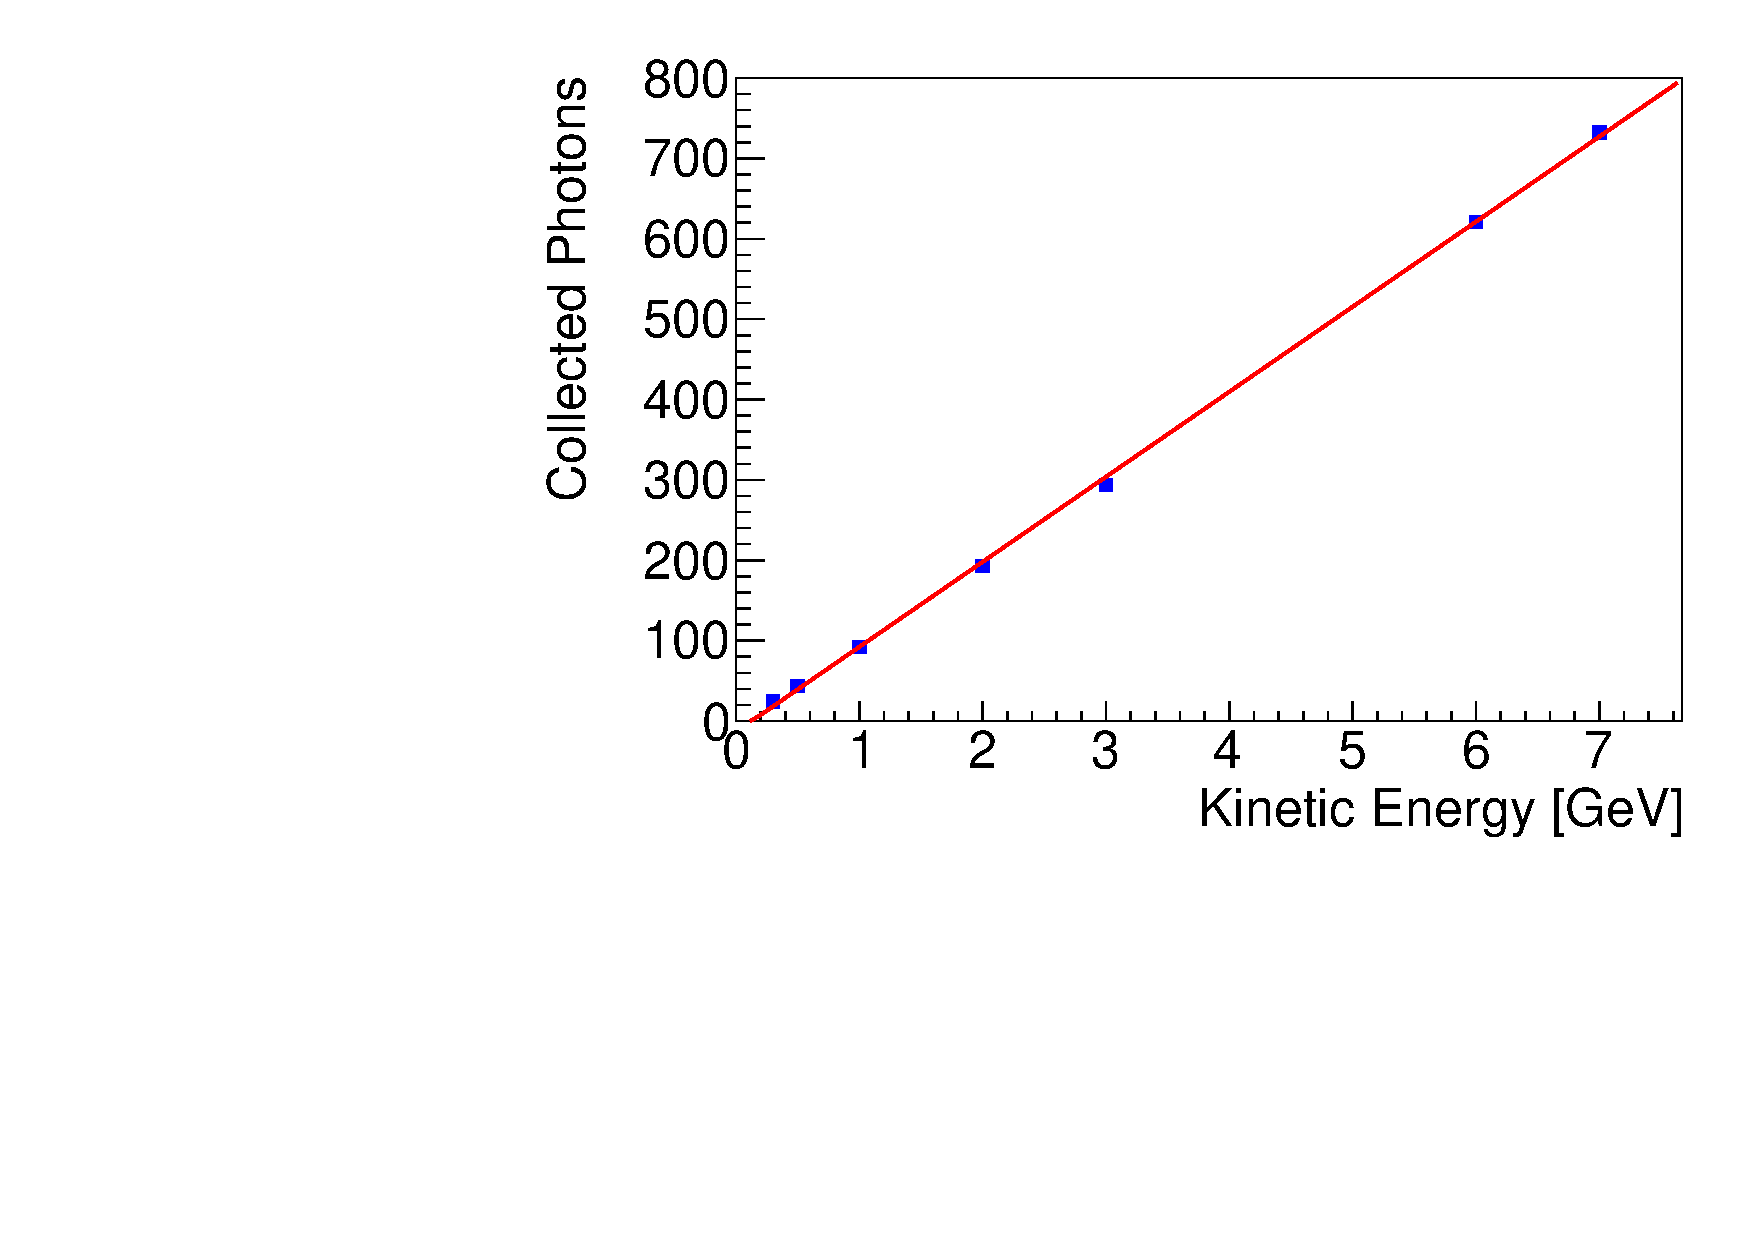
\includegraphics[width=0.5\linewidth]{pdsarapucabeamresponse.pdf}
\end{dunefigure}


The \dword{pdsp} beam run provides a unique set of high quality data for detector performance characterization, physics studies, and calibration. The data will also
allow us to perform hadron-argon cross section measurements, which are relevant for future \dword{dune} neutrino oscillation analyses.
Data collected during the beam run are also used to characterize the \dword{pds} response to light signals. Other useful data sets include
beam data with triggers determined by the beam instrumentation; cosmic-ray data  from random triggers or from those in coincidence with the \dword{crt} modules; and calibration data, with triggers enabling programmed light pulses. 
The single avalanche response and gain for each of the 256 readout channels of the \dword{pds} have been determined from calibration data.
The initial analysis results illustrate very good performance and stability for this system.

Figure~\ref{fig:pdtpcpd} (right) shows the response of an %ARAPUCA photon-detector 
\dword{xarapu} \dword{pd} module as a function of incident electron kinetic energy.
The observed number of photons has not been corrected for geometry and detection efficiency. The analysis demonstrates the achieved energy linearity for beam electrons contained in the detector.  
In addition to explaining the \dword{pds} response and calibration, \dword{pdsp} showed excellent correlation between \dword{tpc} timing and the \dword{pds} timing. The latter will lead to the further optimized physics reach of \dword{dune}. 


\subsection{Near Detector}
\label{sec:nd-verview}


The \dword{dune} \dword{nd} is crucial for the success of the \dword{dune} physics program. It precisely measures the neutrino beam flux and flavor composition. Comparing the measured neutrino energy spectra at the near and far sites allows us to disentangle the different energy-dependent effects that modulate the beam spectrum and to reduce the systematic uncertainties to the level required for discovering \dword{cp} violation. In addition, it will measure neutrino-argon interactions with high precision using both gaseous and liquid argon, which will further reduce the systematic uncertainties due to modelling these interactions.


The \dword{nd} hall will be located \SI{574}{m} downstream from the target and will include three primary detector components, shown in Figure~\ref{fig:neardetectors}  and listed in Table~\ref{tab:NDsumm-esch1}. Two of them can move off beam axis, providing access to different neutrino energy spectra. The movement off axis, called \dword{duneprism}, provides a crucial extra degree of freedom for the \dword{nd} measurement and is therefore an integral part of the \dword{dune} \dword{nd} concept. 


\begin{dunefigure}[DUNE near detector]
{fig:neardetectors}
{\dword{dune}{} Near Detector. The beam enters from the right and encounters
the \dword{lartpc}, the \dword{mpd}, and the on-axis beam monitor with the 3DST.}
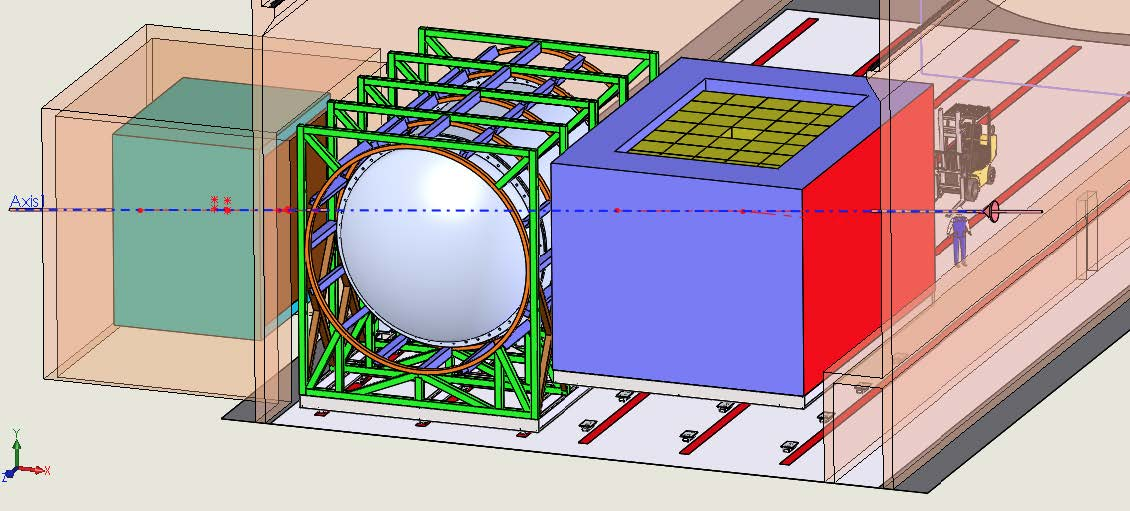
\includegraphics[width=0.9\textwidth]{ND_Detectors.jpg}
\end{dunefigure}

The three detector components (\dword{lartpc} called \dword{arcube}; a \dword{hpgtpc} within a magnet surrounded by an \dword{ecal}, together called \dword{mpd}; and an on-axis beam monitor containing a \dword{3dst} surrounded by the KLOE magnet) \fixme{Is KLOE in the glossary?} serve important individual and overlapping functions in the mission of the \dword{nd}. 
The \dword{dune} \dword{nd} is shown schematically in the \dword{dune} \dword{nd} hall in Figure~\ref{fig:neardetectors}.  
Table~\ref{tab:NDsumm1} provides a high-level overview of the three components of the \dword{dune} \dword{nd} along with the off-axis capability.  

\begin{dunetable}[Components of the DUNE ND]
{p{.22\textwidth}p{.22\textwidth}p{.22\textwidth}p{.22\textwidth}}
{tab:NDsumm-esch1}{This table gives a high-level breakdown of the three major detector components and the capability of movement for the \dword{dune}{} \dword{nd}{} along with function and primary physics goals.}
Component & Essential Characteristics & Primary function & Select physics aims \\ \toprowrule
LArTPC (ArgonCube) & Mass  & Experimental control for the Far Detector & $\numu$($\overline{\nu}_{\mu}$) CC \\
          & Target nucleus Ar &  Measure unoscillated $E_\nu$ spectra   & $\nu$-e$^{-}$ scattering   \\
          &  Technology FD-like    &  Flux determination  &  $\nue +$$\overline{\nu}_{e}$ CC  \\
          &  &  &  Interaction model \\ \colhline
Multipurpose detector (MPD) & Magnetic field & Experimental control for the LArTPCs & $\numu$($\overline{\nu}_{\mu}$) CC \\
  &  Target nucleus Ar & Momentum analyze liquid Ar $\mu$ & $\nue$ CC, $\overline{\nu}_{e}$ \\
  & Low density & Measure exclusive final states with low momentum threshold & Interaction model \\  \colhline
DUNE-PRISM (capability) & LArTPC$+$MPD move off-axis & Change flux spectrum &  Deconvolve flux $\times$ cross section \\ 
 & & & Energy reponse \\
 & & & Provide FD-like energy spectrum at ND\\ 
% & & & {\   }differences \\
 & & & ID mismodeling \\ \colhline
%\dword{3dsts} 
3DST-S & On-axis & Beam flux monitor &  On-axis flux stability \\ 
  & High mass CH target & Neutrons & Interaction model \\ 
& KLOE magnet &  & A dependence \\
    &  & & $\nu$-e$^{-}$ scattering \\ 
\end{dunetable}

The \dword{arcube} detector contains the same target nucleus and shares some aspects of form and functionality with the \dword{fd}. The differences are necessitated by the expected high intensity of the neutrino beam at the \dword{nd}.  This similarity in target nucleus and, to some extent, technology, reduces sensitivity to nuclear effects and detector-driven systematic uncertainties in extracting the oscillation signal at the  \dword{fd}. Using the same target nucleus is particularly important because extrapolation of cross sections between nuclear targets with different atomic number is highly model-dependent. The \dword{lartpc} is large enough to provide high statistics ($\num{1e8}{\numu \text{ charged current events/year}}$), and its volume is sufficiently large to provide good hadron containment.  The tracking and energy resolution, combined with the mass of the \dword{lartpc}, will allow measuring the flux in the beam using several techniques, including the well understood but rare process of $\nu$-e$^{-}$ scattering.

\begin{dunefigure}[DUNE ND Hall with component detectors]
{fig:NDHallconfigs}
{\dword{dune} \dword{nd} hall shown with component detectors all in the on-axis configuration (left) and with the \dword{lartpc} and \dword{mpd} in an off-axis configuration (right). The \dword{3dsts} is shown in position on the beam axis. The beam axis is shown.  The beam enters the hall at the bottom moving from right to left.}
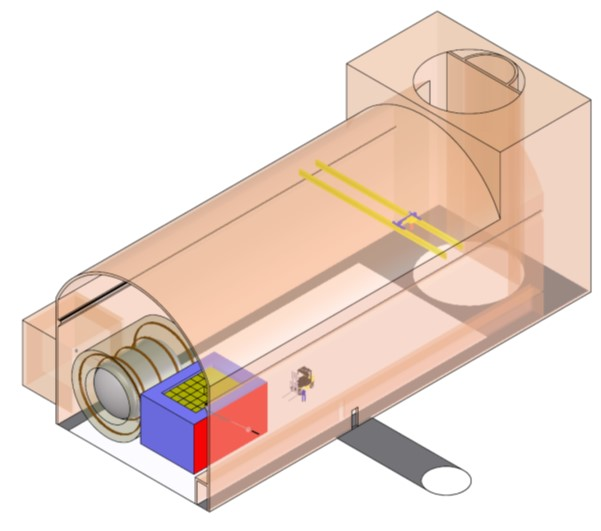
\includegraphics[width=0.49\textwidth]{graphics/NDHall_onaxis.jpg}
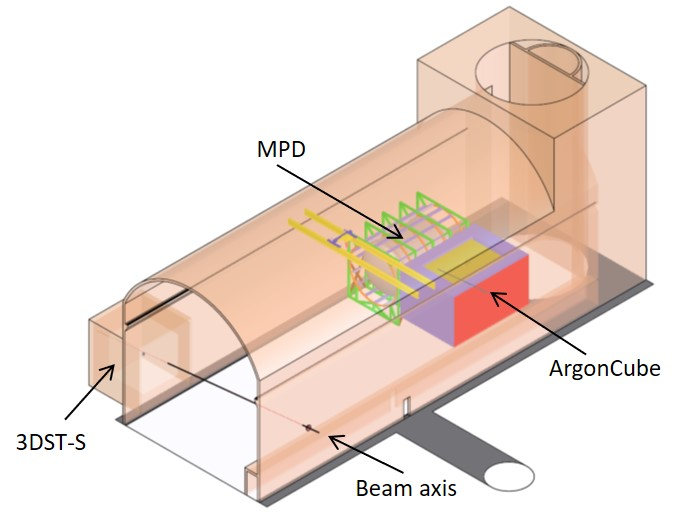
\includegraphics[width=0.49\textwidth]{graphics/NDHall_offaxis.jpg}
\end{dunefigure}

The \dword{lartpc} begins to lose acceptance for muons at a momentum higher than 
$\approx$0.7~GeV/c because muons will not be contained in the \dword{lartpc} volume.  Because muon momentum is critical to determining neutrino energy, a magnetic spectrometer is needed downstream of the \dword{lartpc} to measure the charge sign and momentum of the muons.  In the \dword{dune} \dword{nd} concept, this function is accomplished by the \dword{mpd}, which consists of a \dword{hpgtpc} surrounded by an \dword{ecal} in a \SI{0.5}{T} magnetic field. The \dword{hpgtpc} provides a lower density medium with excellent tracking resolution for muons from the \dword{lartpc}.  

In addition, neutrinos interacting with the argon in the gas \dword{tpc} constitute a sample of $\nu$-argon events that can be studied with a very low charged-particle tracking threshold and excellent resolution superior to \dword{lar}. The high pressure yields a sample of 
$\num{2e6}\,{\numu \text{-CC events/year}}$ for these studies. These events will be valuable for studying charged particle activity near the interaction vertex because this detector can access lower momenta protons than the \dword{lar} detector and can better identify charged pions.  The lack of secondary interactions in these samples will help in identifying the particles produced in the primary interaction and in modeling secondary interactions in denser detectors, which are known to be important \cite{Friedland:2018vry}.

The \dword{lartpc} and \dword{mpd} can be moved sideways up to 33 m to take data in positions off the beam axis.  This capability is referred to as \dword{duneprism}. As the detectors move off-axis, the incident neutrino flux spectrum changes, with the mean energy dropping and the spectrum becoming more monochromatic.  Although the neutrino interaction rate drops off-axis, the intensity of the beam and the size of the \dword{lartpc}  combine to yield ample statistics even in the off-axis positions.
The \dword{dune} concept is based on reconstructing the energy-dependent neutrino spectrum and
comparing the far and near sites. The ability to modify the energy spectrum at the near site by measuring at the off-axis locations will allow disentangling otherwise degenerate effects due to systematic biases of the energy reconstruction.

The final component of the \dword{dune} \dword{nd} suite is the on-axis beam monitor, which contains the
\dword{3dsts} tracker within the magnet of the KLOE detector.  The \dword{3dst} is a plastic scintillator detector made of \SI{1}{cm} cubes read out along each of three orthogonal dimensions.  
This device serves as a dedicated  neutrino spectrum monitor that stays on-axis  when the \dword{lartpc} and \dword{mpd} have moved to an off-axis position. 
It also provides an excellent on-axis neutrino flux determination that can be used as an important point of comparison and a systematic crosscheck for the flux as determined by the \dword{lartpc}.

Chapter~\ref{ch:exsum-nd} of this \dword{tdr} volume presents a more complete introduction to the \dword{nd} and further details of the system can be found in the appendices. 

%%%%%%%%%%%%%%%%%%%%%%%%%%%%%%%%
\section{International Organization and Responsibilities}

\dword{dune} is the first science project in the USA of this scale built with so much
international participation and as an international collaboration. As such, \dword{dune} requires a new organizational and governance model that takes into account the international nature of the project.
The
model used by \dword{cern} to manage constructing and operating the \dword{lhc} and its experiments served as a starting point for the joint management of \dword{lbnf} and the \dword{dune} experimental program.  
\dword{lbnf}, which is responsible for the facilities that comprise the neutrino beam, the near site at \dword{fnal}, and the far site at \surf{}, is organized as a
\dword{doe}-\dword{fnal} project incorporating international partners. 
\dword{dune} is a fully international project
organized by the \dword{dune} collaboration with appropriate oversight from all international stakeholders.
The \dword{dune} collaboration is responsible for
\begin{itemize}
\item the definition of the scientific goals and corresponding scientific and technical requirements of the detector systems and neutrino beamline;
\item the design, construction, commissioning, and operation of the detectors; 
\item the scientific research program conducted with the \dword{dune} detectors. 
\end{itemize}

A set  of  organizational structures  has been established  to
coordinate  the  participating  funding agencies,
overseeing the \dword{lbnf} and \dword{dune} projects,
and coordinating and communicating between the 
two. These structures and the relationships among them are shown 
in Figure~\ref{fig:org}. They include %comprise 
the following committees:
\begin{itemize}
\item International Neutrino Council 

The \dword{inc} is part of the international project governance structure for the  \dword{lbnf} and the  \dword{pip2} projects. The \dword{inc} comprises representatives from the international funding agencies and  \dword{cern} that make major contributions to the infrastructure. 
The \dword{inc} acts as the highest-level international advisory body to the U.S. \fixme{Again, this abbreviation varies from one place to another. Which is the preferred abbreviation? US? U.S.? USA?} \dword{doe} and the  \dword{fnal} directorate on anything related to the program, including coordination among the international partners. The associate director for HEP in the \dword{doe} Office of Science chairs the \dword{inc}, and the \dword{inc}{} includes the  \dword{fnal} director as a member. The council meets once a year and provides pertinent advice on the \dword{lbnf} and \dword{pip2}  projects.
%The council  includes  regional representatives like \dword{cern} and representatives of funding agencies making major contributions to \dword{lbnf} infrastructure and to \dword{dune}. The council acts as the highest-level international advisory body to the U.S. \dword{doe} and the \dword{fnal} directorate. The council facilitates high-level global coordination across the entire enterprise (\dword{lbnf} and \dword{dune}), is chaired by the \dword{doe} Office of Science associate director for high energy physics, and includes the \dword{fnal} director in its membership. The council meets and provides pertinent advice on the \dword{lbnf} and \dword{dune} projects through the \dword{fnal} director as needed.

\item Resources Review Board (RRB)

The \dword{dune}  \dword{rrb} is part of the international project governance structure for the   experiment, established to coordinate among funding partners and oversee \dword{dune}. It has representatives of all funding agencies that sponsor the project and  of \dword{fnal} management. The  \dword{rrb} provides focused monitoring of the \dword{dune} collaboration and also receives updates on the progress of \dword{lbnf},  \dword{pip2}, and the \dword{sbn} programs. The  \dword{rrb} receives periodic reports from both \dword{lbnc} and \dword{ncg}, which are review committees for \dword{dune} charged by and reporting to the \dword{fnal} directorate. A representative from the \dword{fnal} directorate chairs the \dword{rrb} and calls regular meetings to monitor progress on the \dword{dune} project.

%The \dword{rrb} has representatives from all funding agencies that sponsor \dword{lbnf}, \dword{dune}, and \dword{pip2}, and the \dword{fnal} management. The \dword{rrb} provides focused monitoring and detailed oversight of the \dword{dune} collaboration and monitors the progress of \dword{lbnf} and \dword{pip2}. The \dword{fnal} director,  in consultation with the international funding partners for the projects, defines the membership of the \dword{rrb}. A representative from the \dword{fnal} directorate chairs the board and organizes regular meetings for coordinating and to monitoring progress on the projects. The management teams from the \dword{dune} collaboration and the \dword{lbnf} project participate in board meetings and make regular reports to the \dword{rrb} on technical, managerial, financial, and administrative matters, and also report on the status and progress of the \dword{dune} collaboration.

\item Long-Baseline Neutrino Committee (LBNC)

The \dword{fnal} director has charged the \dword{lbnc} to review the scientific, technical, and managerial progress, as well as plans and decisions associated with \dword{dune}. The committee chair reports to the \dword{fnal} director. 
The  \dword{lbnc}, comprising internationally prominent scientists with relevant expertise, 
provides regular external scientific peer review of \dword{dune}. It also provides regular reports and candid assessments to the \dword{fnal} director, which are also available to the \dword{rrb}, \dword{lbnf}, and \dword{dune} leadership, as well as the funding agencies that support these international projects. The  \dword{lbnc} will review the \dword{tdr} for \dword{dune} and recommend endorsing the  \dword{tdr} to the \dword{fnal} directorate and the \dword{rrb}. Upon a request from the \dword{fnal} director, the  \dword{lbnc} may task other \dword{dune} and \dword{lbnf} groups to provide more detailed reports and evaluations of specific systems. The chair of the  \dword{lbnc} will participate as a delegate to both the \dword{fnal}-managed \dword{rrb} and the \dword{doe}-managed \dword{inc}. At meetins of the \dword{rrb} and \dword{inc}, the \dword{lbnc} chair will provide reports on  \dword{lbnc} deliberations to the international delegates. The chair of the  \dword{lbnc} is an ex-officio member of  \dword{fnal}'s Physics Advisory Committee.

%The \dword{lbnc} is composed of internationally prominent scientists with relevant expertise. It provides regular external scientific peer review of \dword{dune} and provides regular reports to the \dword{fnal}  directorate and the \dword{rrb}. The \dword{lbnc} reviews the scientific, technical, and managerial decisions on the \dword{dune} experiment and will review the \dword{tdr} for \dword{dune}, providing a recommendation to the \dword{fnal} directorate and the \dword{rrb} on whether to endorse the \dword{tdr}. Upon request from the \dword{fnal} director, the \dword{lbnc} may task other \dword{dune} and \dword{lbnf} groups to provide more detailed reports and evaluations of specific systems.

\item Neutrino Cost Group (NCG)

The \dword{fnal} director has charged the \dword{ncg} to review the cost, schedule, and associated risks of the \dword{dune} experiment and to provide regular reports to the \dword{fnal} directorate and the \dword{rrb}. This group comprises internationally prominent scientists with relevant experience. 
The  \dword{ncg} will review the  \dword{tdr} for \dword{dune} and will provide a recommendation to the \dword{fnal} directorate and the \dword{rrb} on endorsing the  \dword{tdr}. The chair of the  \dword{ncg} will participate as a delegate to both the \dword{fnal}-managed \dword{rrb} and \dword{doe}-managed \dword{inc}. At meetings of the \dword{rrb} and \dword{inc}, the \dword{ncg} chair will provide reports on  \dword{ncg} deliberations to the international delegates.

%Like the \dword{lbnc}, the \dword{ncg} comprises internationally prominent scientists with relevant experience.  The \dword{ncg} reviews the cost, schedule, and associated risks for the \dword{dune} experiment and provides regular reports to the \dword{fnal} directorate and the \dword{rrb}.  The \dword{ncg} will review the \dword{tdr} for \dword{dune} and will provide a recommendation to the \dword{fnal} directorate and the \dword{rrb} on whether to endorse the \dword{tdr}.


\item Experiment-Facility Interface Group (EFIG)

Coordination between \dword{dune} and \dword{lbnf} must be close and continuous to ensure the success of the combined enterprise. The \dword{efig}  oversees coordination between the two projects, especially during design and construction as well as the operation of the program.   
This group examines interfaces between the detectors and their corresponding conventional facilities, between individual detector systems and the \dword{lbnf} infrastructure, and between design and operation of the \dword{lbnf} neutrino beamline,  which may have issues that affect both \dword{lbnf} and \dword{dune}.  

\end{itemize}

\begin{dunefigure}[Structure for oversight of the DUNE and LBNF projects]	
{fig:org}{Top-level organization structure for oversight of the \dword{dune}{} and \dword{lbnf}{} projects.}
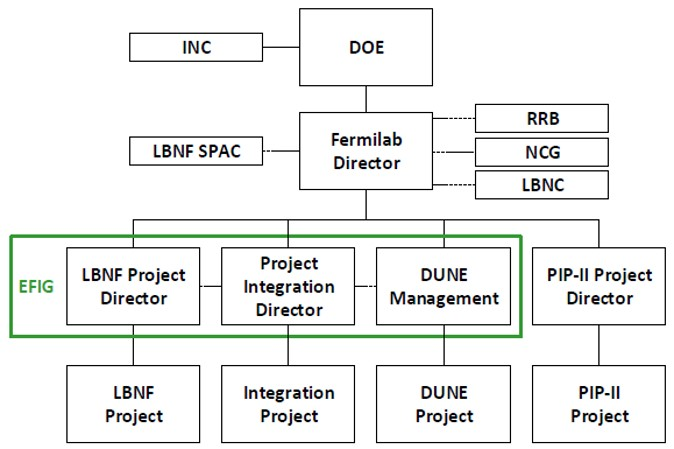
\includegraphics[width=0.67\textwidth]{graphics/lbnf_dune_org.png}  
\end{dunefigure}

\section{DUNE Organization and Management}

The \dword{dune} collaboration organizes and manages \dword{dune} in its entirety.  Stakeholders include all collaborating institutions, including \dword{cern}, the funding agencies participating in \dword{dune}, and \dword{fnal} as the host laboratory.  All collaborating institutions have a representative on the \dword{dune} institutional board. The collaboration is responsible for the design, construction, installation, commissioning, and operation of the detectors and prototypes used to pursue the scientific program. The \dword{dune} executive board, described below, is the main management body of the collaboration and approves all significant strategic and technical decisions.

The top-level \dword{dune} management team consists of two elected co-spokespersons, the \dword{tcoord}, and the \dword{rcoord}. The \dword{tcoord} and \dword{rcoord} are selected jointly by the co-spokespersons and the \dword{fnal} director. The management team is responsible for the day-to-day management of the collaboration and for developing the overall collaboration strategy, which is presented for approval to the executive board. The executive board comprises the leaders of the main collaboration activities. The composition of the executive board, currently including the \dword{dune} management team, institutional board chair, physics coordinator, beam interface coordinator, computing coordinator, \dword{nd} coordinator, and leaders of the \dword{fd} consortia, described below, should ensure
that all stakeholders in the collaboration have a voice in making decisions (see Figure~\ref{fig:eb}). 
Once the \dword{dune} \dword{tdr} is accepted, consortium leaders and coordinators of other major collaboration activities will become elected positions.


\begin{dunefigure}[DUNE executive board]	
{fig:eb}{\dword{dune}{} Executive Board.}
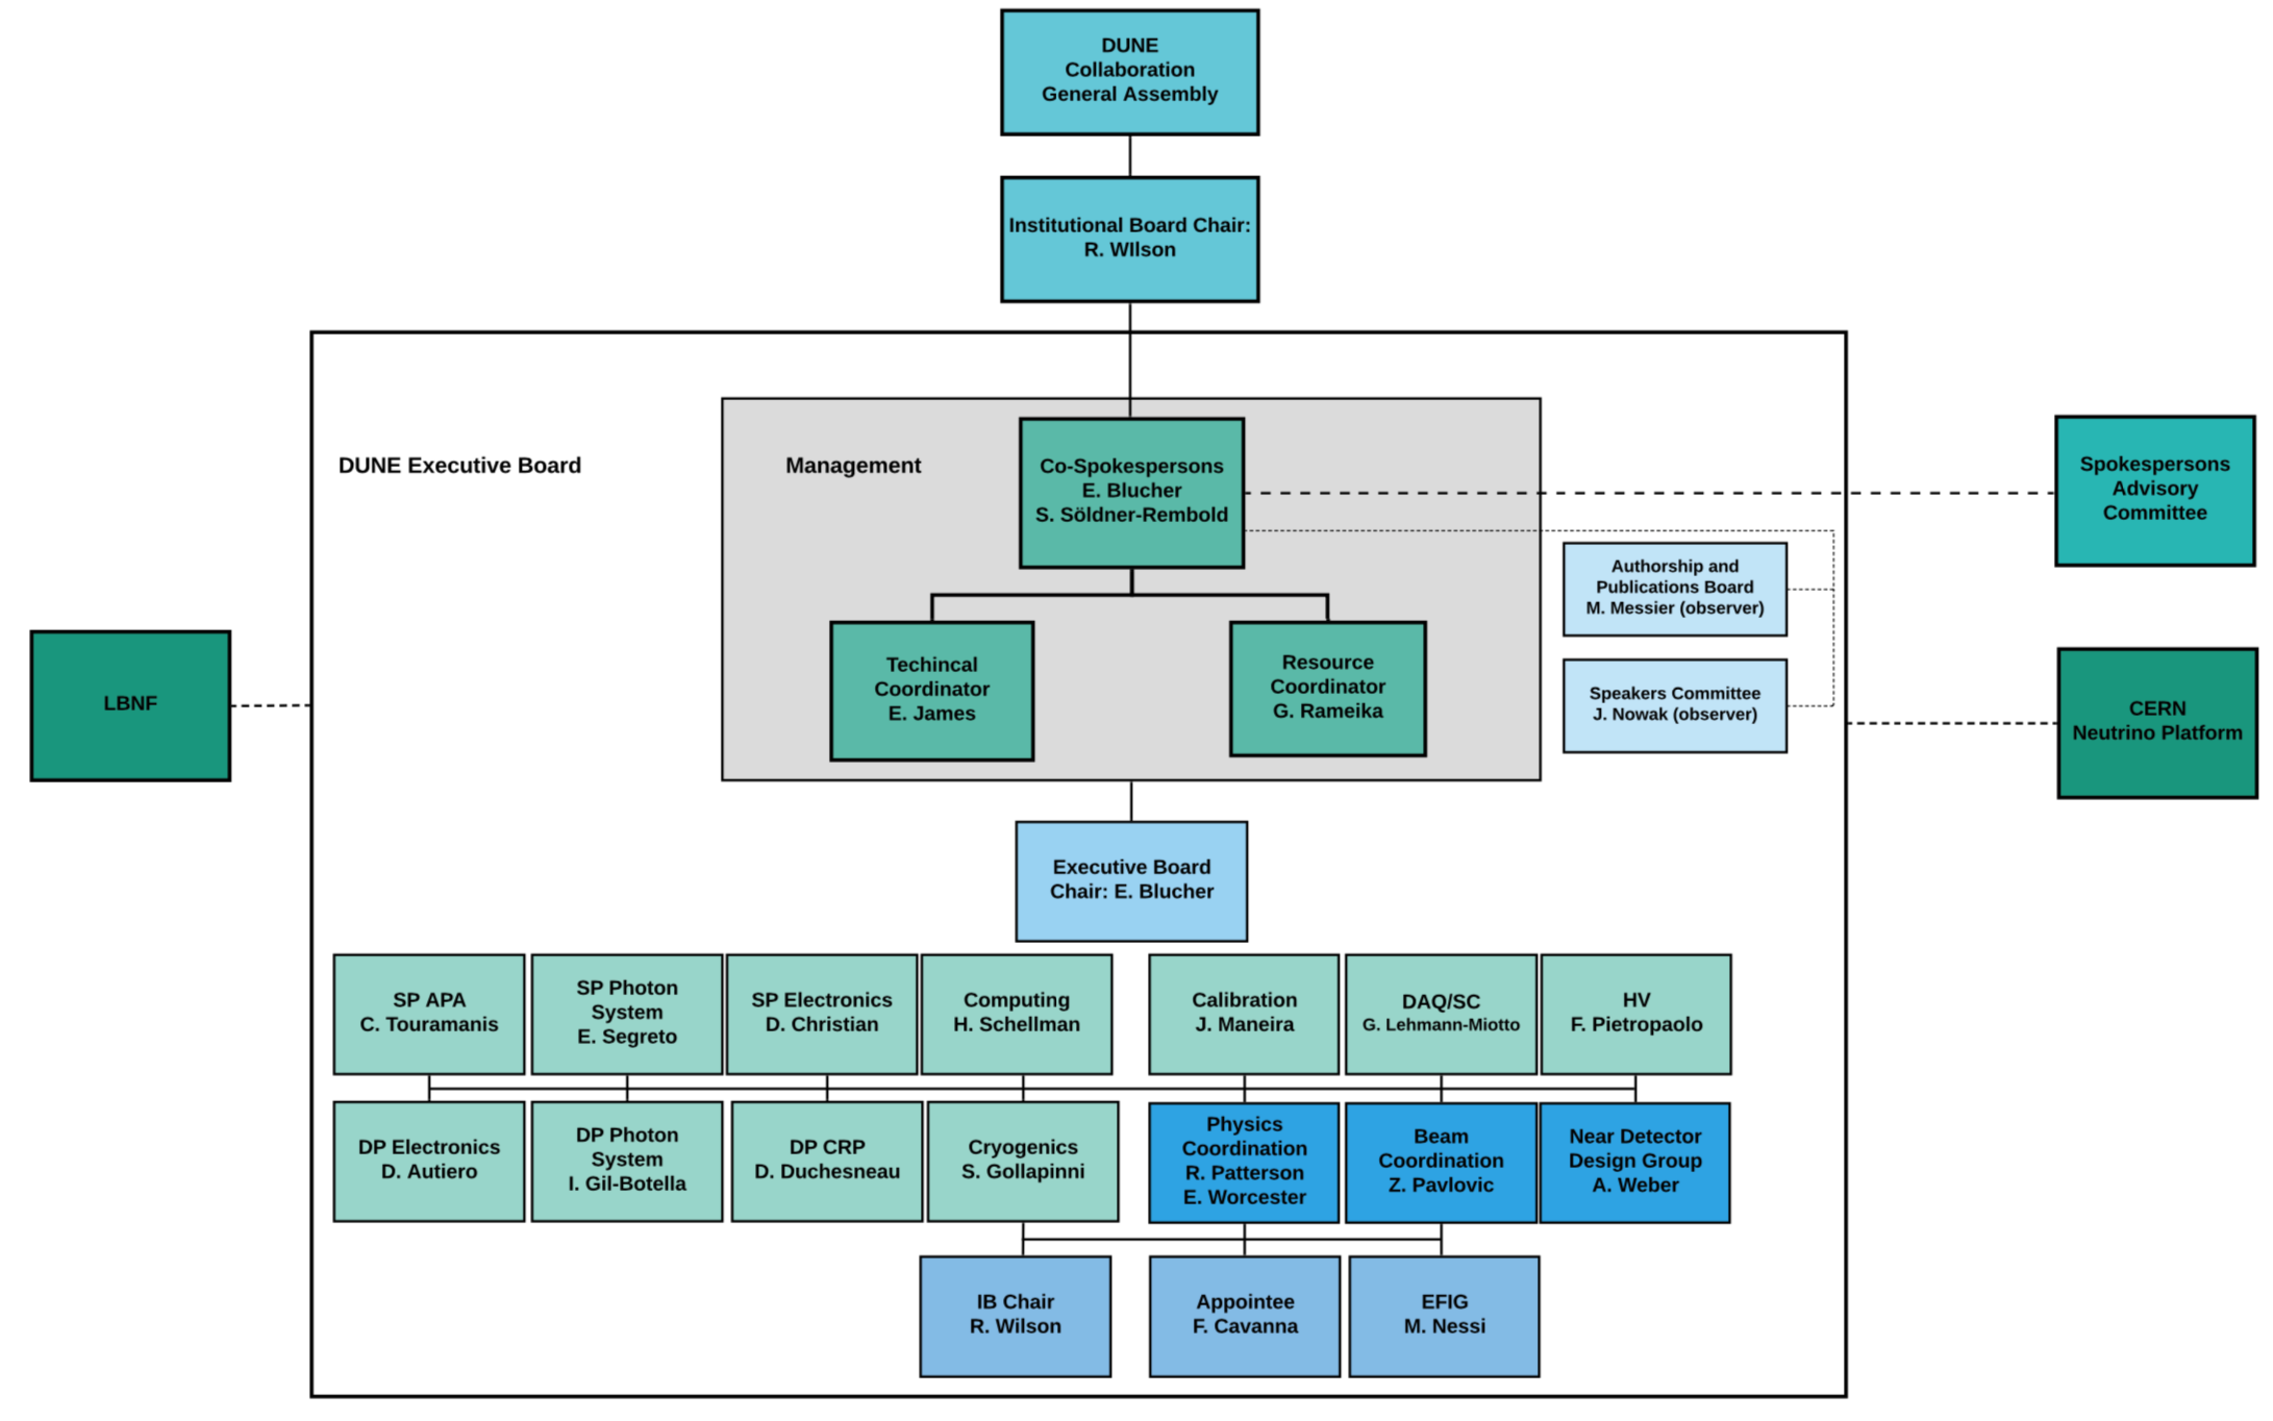
\includegraphics[width=0.9\textwidth]{graphics/eb.pdf}
\end{dunefigure}

To carry out design and construction work for the \dword{dune} \dword{fd}, \dword{dune} has  formed consortia of institutions that are responsible for different detector subsystems. A similar structure will be formed for the \dword{dune} \dword{nd} once the detector concept is selected. The \dword{dune} \dword{fd} currently includes nine consortia, including three specific to \dword{sp}, three specific to \dword{dp}, and five common to both technologies:
\begin{itemize}
\item (\single) \dword{apa}s, %Anode Plane Assemblies% (C. Touramanis, UK)
\item (\single) \dword{tpc} electronics, %\dword{ce}, % (D. Christian, US)
\item (\single) \dword{pds}, %Photon Detection System% (E. Segreto, Brazil)
\item (\dual) \dwords{crp}, %Charge Readout Planes% (D. Duchesneau, France)
\item (\dual) \dword{tpc} electronics, %(D. Autiero, France)
\item (\dual) \dword{pds}, %(PDS), %Photon Detection System %(I. Gil-Botella, Spain)
\item (common) \dword{hvs}, %system, %(F. Pietropaolo, CERN)
\item (common) \dword{daq},  %system, %DAQ System %(D. Newbold, UK)
\item (common) \dword{cisc}, %system, %Slow Controls and Instrumentation. %(S. Gollapinni, US)
\item (common) calibration,  and %system, and
\item (common) computing.
\end{itemize} 
 Each consortium has an overall leader, a technical lead, and a consortium board with representatives from each consortium institution. The consortia have full responsibility for their subsystems and for developing a \dword{wbs}, understanding and documenting all interfaces with other systems, preparing final technical designs, and writing their own sections of the \dword{tdr}. Following approval of the  \dword{tdr}, they will be responsible for constructing their detector systems. %In addition to a variety of other tasks, the consortia are responsible for writing their respective sections of the technical proposal and the TDR.

Chapter~\ref{ch:exec-tc} of this volume provides a more complete introduction to \dword{dune} management and organization; and Volume~\volnumbertc{} of the \dword{tdr} provides still more detail.

%%%%%%%%%%%%%%%%%%%%%%%%%%%%%%%%%%%%%%%%%%%%%%%%%%%%%%%%%%%%%%% new 15 May
\section{Schedule and Milestones} 

The plan includes a set of key milestones and dates and can be found in the \dword{tdr}.  The dates will be final once the international project baseline is established.  Table~\ref{tab:es-key-dates} shows the key dates and milestones (colored rows) and indicates how the detector consortia will add subsystem-specific milestones based on these dates (no background color).
 
\begin{dunetable}
[Key milestones and dates]
{p{0.65\textwidth}p{0.25\textwidth}}
{tab:es-key-dates}
{(Sample subsystem) construction schedule milestones leading to commissioning the first two  \dword{fd}{} modules. Key \dword{dune}{} dates and milestones, found in this \dword{tdr}{}, are shown in orange.  Dates will be final once the international project baseline is established.}   
Milestone & Date (Month YYYY)   \\ \toprowrule
Technology Decision Dates &   April 2020   \\ \colhline
Final Design Review Dates &   June 2020   \\ \colhline
Start of module 0 component production for \dshort{protodune2} & August 2020  \\ \colhline
End of module 0 component production for \dshort{protodune2} & January 2021  \\ \colhline
\rowcolor{dunepeach} Start of \dshort{pdsp}-II installation& \startpduneiispinstall      \\ \colhline
\rowcolor{dunepeach} Start of \dshort{pddp}-II installation& \startpduneiidpinstall      \\ \colhline
\rowcolor{dunepeach}South Dakota Logistics Warehouse available& \sdlwavailable      \\ \colhline
 \dword{prr} dates &  September 2022    \\ \colhline
\rowcolor{dunepeach}Beneficial occupancy of cavern 1 and \dword{cuc}& \cucbenocc      \\ \colhline
Start procurement of (subsystem) hardware & December 2022 \\ \colhline
\rowcolor{dunepeach} \dshort{cuc} counting room accessible& \accesscuccountrm      \\ \colhline
\rowcolor{dunepeach}Top of \dshort{detmodule} \#1 cryostat accessible& \accesstopfirstcryo      \\ \colhline
\rowcolor{dunepeach}Start of \dshort{detmodule} \#1 \dshort{tpc} installation& \startfirsttpcinstall      \\ \colhline
\rowcolor{dunepeach}Top of \dshort{detmodule} \#2 cryostat accessible& \accesstopsecondcryo      \\ \colhline
\rowcolor{dunepeach}End of \dshort{detmodule} \#1 \dshort{tpc} installation& \firsttpcinstallend      \\ \colhline
 \rowcolor{dunepeach}Start of \dshort{detmodule} \#2 \dshort{tpc} installation& \startsecondtpcinstall      \\ \colhline
\rowcolor{dunepeach}End of \dshort{detmodule} \#2 \dshort{tpc} installation& \secondtpcinstallend      \\  \colhline
Full  (subsystem) commissioned and integrated into remote operations & July 2026 \\ 
\end{dunetable}


The schedule for the design and construction of \dword{lbnf} and \dword{dune} has two critical parallel paths: one for the %Far Site scope at SURF 
far site (South Dakota) %(\surf) and %one 
and another for the %Near Site scope at 
near site (Illinois). %(\dword{fnal}). 
The schedule for initial work is driven by the design and construction of the \dword{cf} (conventional facilities).

During the initial phase of the project, the far site \dword{cf} comes first. 
%The Ross Shaft rehabilitation work at \dword{surf} was recently halted at the 4850 level because of safety concerns that led to delays of two to four months. 
Early site preparation should be complete 
before excavation begins, once Ross Shaft rehabilitation work is done. As each detector 
 cavern is excavated and sufficient utilities are installed, the cryostat and cryogenics system work begins, followed by detector installation, filling, and commissioning. 
The first \dword{detmodule} should be operational by 2024, with the second module completed one year later in 2025 and the third in 2027.

\dword{doe} project management requires approval at critical decision milestones before allowing the \dword{lbnf}/\dword{dune} project to move on to the next step. 
CD-1R was granted in 2015, and CD-3A for \dword{lbnf} far site construction was granted in 2016. 
In spring 2020, \dword{dune} and \dword{lbnf} will seek CD-2/3b,  and 
in fall 2020, \dword{dune} and \dword{lbnf} will seek CD-2/3 for the near site. 
The project concludes with CD-4 approval to start operations.

%%%%%%%%%%%%%%%%%%%%%%%%%%%%%%%%%%%%%%%%%%%%%%%%%%%%%%%%%%%%%%
\section{Organization of the DUNE Technical Design Report}

The \dword{dune} \dword{tdr} describes the experiment's proposed physics program, the 
technical designs of the two \dword{fd} \dword{lartpc} technologies, and the technical coordination required to construct and commission the first far \dwords{detmodule}.
The \dword{tdr} will 
justify the technical choices that flow down from the high-level physics goals through requirements at all levels of the project. These design choices will enable the \dword{dune} experiment to make the ground-breaking discoveries that will help answer 
fundamental physics questions. 

The \dword{dune} \dword{fd} designs have been prototyped with the two \dword{protodune} detectors at \dword{cern}, and these designs, while largely complete, are undergoing adjustments following lessons learned. Producing detector components is being planned. 
The \dword{dune} \dword{tdr}, therefore, presents a final technical design for most elements, as well as the few remaining alternative or enhanced designs under consideration. The \dword{tdr} represents the state of the design for the first three \dword{dune} \dword{fd} modules.
The fourth module could implement a new \dword{lartpc} configuration, taking into account  potential advances in technology to enhance sensitivity for physics discoveries. 
 The \dword{nd} \dword{tdr} is planned for 2020, and the computing \dword{tdr} will be provided on a similar timescale.

The \dword{dune} \dword{fd} \dword{tdr} has five volumes:

\begin{itemize}
\item Volume~\volnumberexec{} provides the executive summary of the overall experimental program. It includes a brief description of the \dword{dune} science program, the \dword{dune} detectors, and technical coordination, which are subjects of the remaining volumes in the \dword{tdr}. This volume also includes a description of two systems not yet at the technical design stage: the \dword{dune} \dword{nd} and \dword{dune} computing.
\item Volume~\volnumberphysics{} outlines the scientific objectives and describes the physics studies that the \dword{dune} collaboration will undertake and the methods for meeting those objectives.
\item Volume~\volnumbersp{} describes the \dword{sp} \dword{fd} technology, subsystems, and components that the first (and any subsequent) \dword{sp} \dwords{detmodule} will comprise, as well as the installation plan for the first \dword{fd} module, which will be of this type. 
\item Volume~\volnumberdp{} describes the \dword{dp} \dword{fd} technology, the subsystems, and components that  the first (and any subsequent) \dword{dp} \dwords{detmodule} will comprise, as well as the installation plan for the first \dword{dp} module. 
\item Volume~\volnumbertc{} describes the organizational structures,  methodologies, procedures, requirements, risks, and other technical  coordination aspects of constructing the first two \dword{fd} modules in South Dakota.
\end{itemize}

